\newpage

\subsection{QuizziPedia::Front-End::Models}

	\label{QuizziPedia::Front-End::Models}
	
	\begin{figure}[ht]
		\centering
		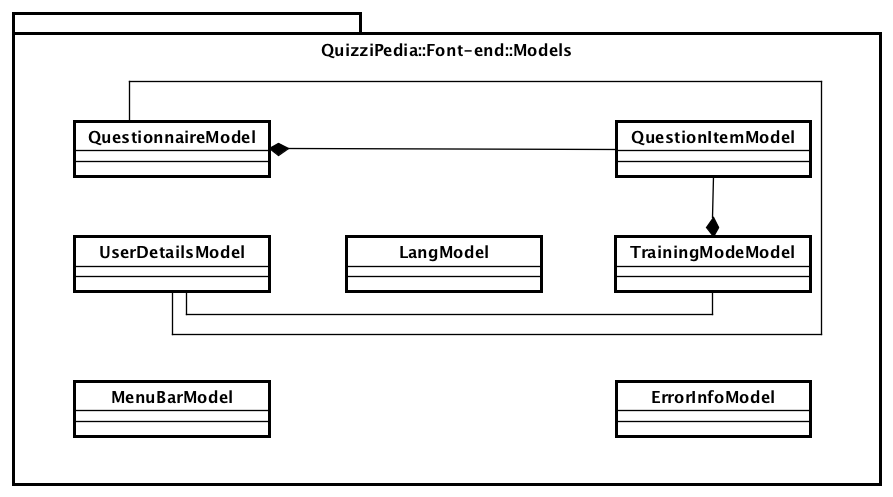
\includegraphics[scale=0.5,keepaspectratio]{UML/Package/QuizziPedia_Front-End_Models.png}
		\caption{QuizziPedia::Front-End::Models}
	\end{figure} \FloatBarrier

		\begin{itemize}
			\item \textbf{Descrizione}: \textit{package\ped{G}} contenente le classi che definiscono la business logic dell'applicazione;
			\item \textbf{Padre}: \texttt{Front-End};
			\item \textbf{Iterazioni con altri componenti}: 
				\begin{itemize}				
					\item \texttt{Controllers}: \textit{package\ped{G}} contenente i controllers front-end dell'applicazione;
					\item \texttt{Directives}: \textit{package\ped{G}} contenente le directives front-end dell'applicazione;
					\item \texttt{Models}: \textit{package\ped{G}} contenente le classi che definiscono la business logic dell'applicazione;
					\item \texttt{Services}: \textit{package\ped{G}} che contiene le classi individuate che permettono la comunicazione del lato front-end con il lato back-end attraverso l'architettura \textit{REST\ped{G}}.
				\end{itemize}
			\item \textbf{Classi contenute}:
			\begin{itemize}
				\item \texttt{UserDetailsModel}: rappresenta un utente. Contiene tutte le informazioni necessarie alla presentazione del contenuto di un utente sia nella visualizzazione che nella gestione di un profilo;
				\item \texttt{TrainingModeModel}: rappresenta un allenamento. Contiene tutte le informazioni necessarie alla presentazione del contenuto di un allenamento;
				\item \texttt{QuestionnaireModel}: rappresenta un questionario. Contiene tutte le informazioni necessarie alla presentazione del contenuto del questionario;
				\item \texttt{QuestionItemModel}: rappresenta una domanda. Contiene tutte le informazioni necessarie alla presentazione del contenuto della domanda;
				\item \texttt{MenuBarModel}: questa classe racchiude i dati necessari per la creazione dinamica della barra menù posizionata in modo fisso su ogni pagina;
				\item \texttt{LangModel}: rappresenta le informazioni per la giusta traduzione dell'applicazione;
				\item \texttt{ErrorInfoModel}: rappresenta le informazioni di un errore che si è verificato eseguendo una determinata operazione;
			\end{itemize}
		\end{itemize}